\documentclass{exam}
%\documentclass[11pt,a4paper]{exam}
\usepackage{amsmath,amsthm,amsfonts,amssymb,dsfont}
\usepackage{ifthen}
\usepackage{graphicx}
\usepackage{geometry}
\geometry{
legalpaper, total={177.8mm, 290mm},left=20mm,
top=7mm, bottom=27mm,
}
\usepackage{enumerate}% http://ctan.org/pkg/enumerate
\usepackage{multicol}
\usepackage{hhline}
\usepackage[table]{xcolor}


% Accumulate the answers. Unmodified from Phil Hirschorn's answer
% https://tex.stackexchange.com/questions/15350/showing-solutions-of-the-questions-separately/15353
\newbox\allanswers
\setbox\allanswers=\vbox{}

\newenvironment{answer}
{%
    \global\setbox\allanswers=\vbox\bgroup
    \unvbox\allanswers
}%
{%
    \bigbreak
    \egroup
}

\newcommand{\showallanswers}{\par\unvbox\allanswers}
% End Phil's answer


% Is there a better way?
\newcommand*{\getanswer}[5]{%
    \ifthenelse{\equal{#5}{a}}
    {\begin{answer}\thequestion. (a)~#1\end{answer}}
    {\ifthenelse{\equal{#5}{b}}
        {\begin{answer}\thequestion. (b)~#2\end{answer}}
        {\ifthenelse{\equal{#5}{c}}
            {\begin{answer}\thequestion. (c)~#3\end{answer}}
            {\ifthenelse{\equal{#5}{d}}
                {\begin{answer}\thequestion. (d)~#4\end{answer}}
                {\begin{answer}\textbf{\thequestion. (#5)~Invalid answer choice.}\end{answer}}}}}
}

\setlength\parindent{0pt}
%usage \choice{ }{ }{ }{ }
%(A)(B)(C)(D)
\newcommand{\fourch}[5]{
    \par
    \begin{tabular}{*{4}{@{}p{0.23\textwidth}}}
        (a)~#1 & (b)~#2 & (c)~#3 & (d)~#4
    \end{tabular}
    \getanswer{#1}{#2}{#3}{#4}{#5}
}

%(A)(B)
%(C)(D)
\newcommand{\twoch}[5]{
    \par
    \begin{tabular}{*{2}{@{}p{0.46\textwidth}}}
        (a)~#1 & (b)~#2
    \end{tabular}
    \par
    \begin{tabular}{*{2}{@{}p{0.46\textwidth}}}
        (c)~#3 & (d)~#4
    \end{tabular}
    \getanswer{#1}{#2}{#3}{#4}{#5}
}

%(A)
%(B)
%(C)
%(D)
\newcommand{\onech}[5]{
    \par
    (a)~#1 \par (b)~#2 \par (c)~#3 \par (d)~#4
    \getanswer{#1}{#2}{#3}{#4}{#5}
}

\newlength\widthcha
\newlength\widthchb
\newlength\widthchc
\newlength\widthchd
\newlength\widthch
\newlength\tabmaxwidth

\setlength\tabmaxwidth{0.96\textwidth}
\newlength\fourthtabwidth
\setlength\fourthtabwidth{0.25\textwidth}
\newlength\halftabwidth
\setlength\halftabwidth{0.5\textwidth}

\newcommand{\choice}[5]{%
\settowidth\widthcha{AM.#1}\setlength{\widthch}{\widthcha}%
\settowidth\widthchb{BM.#2}%
\ifdim\widthch<\widthchb\relax\setlength{\widthch}{\widthchb}\fi%
    \settowidth\widthchb{CM.#3}%
\ifdim\widthch<\widthchb\relax\setlength{\widthch}{\widthchb}\fi%
    \settowidth\widthchb{DM.#4}%
\ifdim\widthch<\widthchb\relax\setlength{\widthch}{\widthchb}\fi%

% These if statements were bypassing the \onech option.
% \ifdim\widthch<\fourthtabwidth
%     \fourch{#1}{#2}{#3}{#4}{#5}
% \else\ifdim\widthch<\halftabwidth
% \ifdim\widthch>\fourthtabwidth
%     \twoch{#1}{#2}{#3}{#4}{#5}
% \else
%      \onech{#1}{#2}{#3}{#4}{#5}
%  \fi\fi\fi}

% Allows for the \onech option.
\ifdim\widthch>\halftabwidth
    \onech{#1}{#2}{#3}{#4}{#5}
\else\ifdim\widthch<\halftabwidth
\ifdim\widthch>\fourthtabwidth
    \twoch{#1}{#2}{#3}{#4}{#5}
\else
    \fourch{#1}{#2}{#3}{#4}{#5}
\fi\fi\fi}


\begin{document}

\begin{table}[h]
\centering
\begin{tabular}{lllll}
\textbf{\large SYLHET CADET COLLEGE} &  &  &  &  \\ \cline{4-5} 
FIRST TERM-END EXAMINATION - 2024 &  & \multicolumn{1}{l|}{} & \multicolumn{1}{l|}{Set} & \multicolumn{1}{l|}{A} \\ \cline{4-5} 
CLASS: XII &  &  &  &  \\ \cline{3-5} 
MULTIPLE CHOICE QUESTIONS & \multicolumn{1}{l|}{\textbf{Subject Code:}} & \multicolumn{1}{l|}{1} & \multicolumn{1}{l|}{3} & \multicolumn{1}{l|}{0} \\ \cline{3-5} 
STATISTICS FIRST PAPER &  &  &  &  \\
TIME – 25 minutes &  &  &  &  \\
FULL MARKS – 25 &  &  &  & 
\end{tabular}
\end{table}
%  \normalfont\normalsize
 % 11.45a.m.~--~1.45p.m.
\hrule

\begin{center}
[N.B. – Answer all the questions. Each question carries ONE mark. Block fully, 
with a black ball- point pen, the circle of the letter that stands for 
the correct/best answer in the “Answer sheet” for the Multiple Choice 
Questions.]\\

  
  \textbf{Candidates are asked not to leave any mark or spot on the question paper.}
\end{center}
\begin{questions}

\question \textbf{What is the value of $\sum (x_i+4)$ if x =\{2,3\}?}
\choice{23}{47}{22}{13}{d}

\question \textbf{Which of the following is an example of an ordinal scale?}  
\choice{Temperature}{IQ Score}{Educational Level}{Weight}{c}

\textbf{Answer the next three questions based on the following information.}

The values of $x_i$ and $f_i$ are given below:

\begin{table}[h]
\centering
\begin{tabular}{c|c|c|c|c}
$x_i$ & 1     & 2     & 3     & 4     \\ \hline
$f_i$ & 2     & 3     & 4     & 1    
\end{tabular}
\end{table}

\question \textbf{Find $\displaystyle \sum_{i=1}^4 f_i x_i$.}  
\choice{20}{21}{22}{24}{d}  

\question \textbf{Compute $\displaystyle \sum_{i=1}^4 f_i x_i^2$.}  
\choice{30}{35}{66}{64}{c}  

\question \textbf{Determine $\displaystyle \sum_{i=1}^4 f_i^2 x_i$.}  
\choice{74}{49}{78}{65}{a}  

\question \textbf{Which measure of central tendency is suitable for qualitative variable?}
\choice{Arithmetic Mean}{Harmonic Mean}{Quadratic Mean}{Mode}{d}

\question \textbf{A good measure of central tendency -}

i. is loosly defined \\
ii. takes into consideration all values \\
iii. easily understandable

\textbf{Which one is correct?}

\choice{i and ii}{i and iii}{ii and iii}{i, ii and iii}{c}

\question \textbf{The Arithmetic Mean of two numbers is 35. If one number is 50, 
what is the other number?}
\choice{25}{20}{40}{70}{b}

\question \textbf{What is the arithmetic mean of first n even natural numbers?}
\choice{$\frac{n+1}{2}$}{$n+1$}{$n$}{$\frac{n-1}{2}$}{b}

\textbf{Answer the next three questions as per the following information.}

\begin{center}
42 44 59 64 70 72 74 91 94 are 9 values.
\end{center}

\question \textbf{What is the median?}
\choice {64}{70}{72}{71}{b}

\question \textbf{What is the first quartile?}
\choice {42.4}{44.7}{51.5}{64.2}{c}

\question \textbf{Above which value lie 60\% observations?}
\choice{70.4}{72.0}{74.6}{66.4}{c}

\question \textbf{First moment around zero is --}
\choice{0}{1}{-1}{Arithmetic Mean}{d}

\question \textbf{The arithmetic mean of a variable is 2.6. What is the 
first raw moment around 6?}
\choice{2.2}{-3.4}{0.1}{1.8}{b}

\question \textbf{For a symmetrical distribution, $\beta_1=--$}
\choice{1}{-1}{0}{3}{c}

\question \textbf{$\gamma_1=0.43$ implies--}
\choice{Left Skew}{Symmetry}{Right Skew}{Mesokurtic}{c}

\textbf{Answer the next THREE questions based on the following information}

\begin{center}
   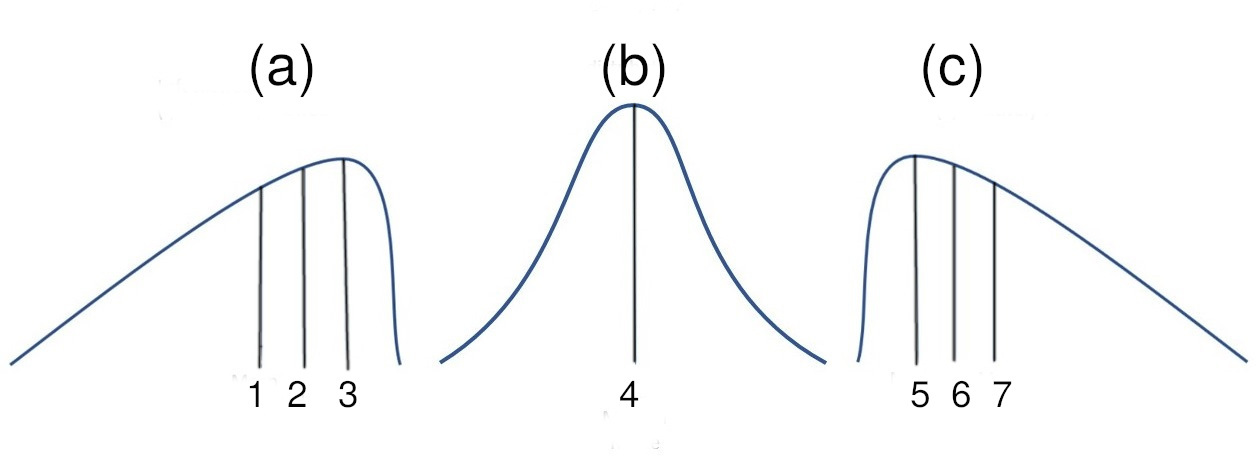
\includegraphics[width=0.5\textwidth]{../../slide/img/skewness_clean.jpg}
\end{center}

\question \textbf{The curve (a) is an example of}
\choice{Positive Skew}{Negative Skew}{No Skew}{Not detectable}{b}

\question \textbf{In Image (b), what is denoted by 4th value?}
\choice{Mean}{Median}{Mode}{All of the above}{d}

\question \textbf{What is the value corresponding to the position 7?}
\choice{Mean}{Median}{Mode}{None of the above}{a}

\question \textbf{In a symmetric distribution--}

i. Frequencies of higher values are lower \\
ii. Frequencies of low values are higher \\
iii. Frequencies of low values are lower 

\textbf{Which one is correct?}

\choice{i and ii}{i and iii}{ii and iii}{i, ii and iii}{b}

\question \textbf{Which is an example of time series data?}
\choice{Number of calls received by a call center each month}
{Height of children at different ages}
{Tota salary of all employees at a company}
{Population of different countries in 2020}{a}

\end{questions}

 \vspace{2.5cm}

\begin{center}
“We are drowning in information and starving for knowledge.” -- 
Rutherford David Rogers
\end{center}

\pagebreak
%\newpage  %Uncomment to put on new age
\bigskip

\begin{multicols}{3}
[
Answer Key
]
\showallanswers % Phil Hirschorn
\end{multicols}


\end{document}